\label{ch:compressible-theory}


%-----------------------------------------------------------------------------
\section{Euler equation properties}

The Euler equations\footnote{ We focus on the Euler equations, which
are the most commonly modeled set of fluid equations in astrophysics.
The more general equation set, the Navier-Stokes equations, includes
dissipative terms.  However, for astophysical flows, the scales on
which these dissipative terms operate are usually much smaller than
the system of interest (equivalently, Reynolds numbers of
astrophysical flows are very large).}  in one dimension appear as:
\begin{align}
\frac{\partial \rho}{\partial t} +
    \frac{\partial (\rho u)}{\partial x} &= 0 \\
%
\frac{\partial(\rho u)}{\partial t} +
    \frac{\partial (\rho uu + p)}{\partial x} &= 0 \\
%
\frac{\partial(\rho E)}{\partial t} +
    \frac{\partial(\rho u E + u p)}{\partial x} &= 0
\end{align}
These represent conservation of mass, momentum, and energy.  Here $\rho$ is the
density, $u$ is the one-dimensional velocity, $p$ is the pressure, and $E$
is the total energy / mass, and can be expressed in terms of the
specific internal energy and kinetic energy as:
\begin{equation}
E = e + \frac{1}{2} u^2
\end{equation}
The equations are closed with the addition of an equation of state.  A common
choice is the gamma-law EOS:
\begin{equation}
p = \rho e(\gamma - 1)
\end{equation}
where $\gamma$ is the ratio of specific heats for the gas/fluid (for
an ideal, monatomic gas, $\gamma = 5/3$), but any relation of the form
$p = p(\rho, e)$ will work.

One thing that we can notice immediately is that there is no need for
temperature in this equation set, although often, when source terms
are present, we will need to obtain temperature from the equation of
state.

In this form, the equations are said to be in {\em conservative form},
i.e.\ they can be written as:
\begin{equation}
U_t + \left [F(U) \right ]_x = 0
\end{equation}
with
\begin{equation}
U = \left ( \begin{array}{c} \rho \\ \rho u \\ \rho E \end{array} \right )
%
\qquad
%
F(U) = \left ( \begin{array}{c} \rho u \\ \rho uu + p \\ \rho u E + up \end{array} \right )
\end{equation}
%
We can write this in {\em quasi-linear} form by first expressing the flux
vector in terms of the conserved variables directly.  Taking
$m \equiv \rho u$, $\mathcal{E} \equiv \rho E$, and expressing
\begin{equation}
p = \rho e (\gamma-1) =  \left (\mathcal{E} - \frac{1}{2} \frac{m^2}{\rho}\right )(\gamma - 1)
\end{equation}
we have
\begin{equation}
F(U) = \left ( \begin{array}{c}
      m \\
      \frac{1}{2}\frac{m^2}{\rho} \left (3 - \gamma \right ) +
          \mathcal{E} (\gamma - 1) \\
      \frac{m\mathcal{E}}{\rho} \gamma -\frac{1}{2} \frac{m^3}{\rho^2} (\gamma -1) \end{array} \right )
\end{equation}
The Jacobian of this flux vector can now be computed as $A = \partial
F/\partial U$:
\begin{equation}
A(U) = \left ( \begin{array}{ccc}
   0  & 1 & 0 \\
   -\frac{1}{2}u^2(3 -\gamma) & u (3 -\gamma) & \gamma - 1 \\
   \frac{1}{2}(\gamma -2)u^3 - \frac{uc^2}{\gamma -1} &
       \frac{3-2\gamma}{2} u^2 + \frac{c^2}{\gamma -1} & u \gamma
  \end{array} \right )
\end{equation}\MarginPar{SymPy notebook?}
where the speed of sound is $c = \sqrt{\gamma p/\rho}$.   With this, our
system can be written as:
\begin{equation}
U_t + A(U) U_x = 0
\end{equation}
This matrix is quite complex and difficult to work with.  The
eigenvectors of this matrix can be found in a variety of sources
(e.g. \cite{toro:1997,athena}).


An alternate way to express these equations is using the {\em
  primitive variables}: $\rho, u, p$.
\begin{exercise}[Primitive variable form of the Euler equations]
{Show that the Euler equations in primitive form can
  be written as
\begin{equation}
q_t + A(q) q_x = 0
\end{equation}
where
\begin{equation}
q = \left ( \begin{array}{c} \rho \\ u \\ p \end{array} \right )
%
\qquad
A(q) = \left ( \begin{array}{ccc} u  & \rho     & 0 \\
                                  0  &  u       & 1/\rho \\
                                  0  & \gamma p & u \end{array} \right )
\label{eq:primitivesystem}
\end{equation}
}
\end{exercise}
%
The eigenvalues of $A$ can be found via $| A - \lambda I | = 0$,
where $|\ldots|$ indicates the determinant and $\lambda$ are the eigenvalues.
\begin{exercise}[The eigenvalues of the Euler system]
{
Show that the eigenvalues of $A$ are $\lambda^\evm = u -c$, $\lambda^\evz = u$, $\lambda^\evp = u+c$.
}
\end{exercise}
Note that both the conserved Jacobian matrix, $A(U)$, and the
primitive variable matrix, $A(q)$, have the same eigenvalues,
 since they represent the same physics.

In Eq.~\ref{eq:primitivesystem}, we used the algebraic gamma-law
equation of state to replace $e$ with $p$, however, for a general
equation of state, we can get the appropriate expression by writing $p
= p(\rho, s)$:
\begin{equation}
\frac{Dp}{Dt} = \left . \frac{\partial p}{\partial \rho} \right |_s
     \frac{D\rho}{Dt} +
     \left . \frac{\partial p}{\partial s} \right |_\rho
     \cancelto{0}{\frac{Ds}{Dt}}
\end{equation}
where $Ds/Dt = 0$ when no entropy sources are present.  Recognizing
that $\Gamma_1 \equiv \partial \log p/\partial \log \rho |_s$, we have:
\begin{equation}
\frac{\partial p}{\partial t} + u \frac{\partial p}{\partial x}
  + \Gamma_1 p \frac{\partial u}{\partial x} = 0  \label{eq:euler:pgeneral}
\end{equation}
as the generalization of the pressure equation.

We'll use the symbols $\{-,\circ,+\}$ to denote the eigenvalues and their
corresponding eigenvectors throughout these notes.
These eigenvalues are the speeds at which information propagates through
the fluid.
Since the eigenvalues are real, this system (the Euler equations) is said
to be {\em hyperbolic}.  Additionally, since $A = A(q)$, the system is
said to be {\em quasi-linear}.
%
The right and left eigenvectors can be found via:
\begin{equation}
A \, r^\enu = \lambda^\enu r^\enu \; ;
\qquad
l^\enu \, A  = \lambda^\enu l^\enu
\end{equation}
where $\nu = \{-,\circ,+\}$ corresponding to the three waves, and
there is one right and one left eigenvector for each of the eigenvalues.
%
\begin{exercise}[Eigenvectors of the Euler system]
{
Show that the right eigenvectors are:
\begin{equation}
r^\evm = \left ( \begin{array}{c} 1 \\ -c/\rho \\ c^2 \end{array} \right )
%
\qquad
r^\evz = \left ( \begin{array}{c} 1 \\ 0 \\ 0  \end{array} \right )
%
\qquad
r^\evp = \left ( \begin{array}{c} 1 \\ c/\rho \\ c^2 \end{array} \right )
\end{equation}
and the left eigenvectors are:
\begin{align}
l^\evm &= \left ( \begin{array}{ccc} 0 & -\frac{\rho}{2c} & \frac{1}{2c^2}
                  \end{array} \right ) \\
%
\qquad
l^\evz &= \left ( \begin{array}{ccc} 1 & 0 & -\frac{1}{c^2}  \end{array} \right ) \\
%
\qquad
l^\evp &= \left ( \begin{array}{ccc} 0 & \phantom{+}\frac{\rho}{2c} & \frac{1}{2c^2} \end{array} \right )
\end{align}
Note that in general, there can be an arbitrary constant in front of each
eigenvector.  Here they are normalized such that
$l^{(i)} \cdot r^{(j)} = \delta_{ij}$.
}
\end{exercise}
A {\sf IPython} notebook using {\sf SymPy} that derives these is available here:
\hydroexdoit{\href{https://github.com/zingale/hydro_examples/blob/master/compressible/euler.ipynb}{euler.ipynb}}
\footnote{if you don't have {\sf IPython}, you can view this rendered online via {\sf nbviewer}:\\
\url{http://nbviewer.ipython.org/github/zingale/hydro_examples/blob/master/compressible/euler.ipynb}}

A final form of the equations is called the {\em characteristic form}.  Here,
we wish to diagonalize the matrix $A$.  We take the matrix $R$ to be the
matrix of right eigenvectors,
\begin{equation}
R = (r^\evm | r^\evz | r^\evp )
\end{equation}
(i.e., $R$ is a square matrix whose columns are the eigenvectors),
and $L$
is the corresponding matrix of left eigenvectors:
\begin{equation}
L = \left ( \begin{array}{c} l^\evm \\
                             \hdashline
                             l^\evz \\
                             \hdashline
                             l^\evp \end{array} \right )
\end{equation}
Note that $L\, R = I = R\, L$, and $L = R^{-1}$.
\begin{exercise}[Characteristic form of the Euler equations]
{
Show that $\Lambda = L A R$ is a diagonal matrix with the diagonal elements
simply the 3 eigenvalues we found above:
\begin{equation}
\Lambda =
   \left ( \begin{array}{ccc}
             \lambda^\evm &              & \\
                          & \lambda^\evz & \\
                          &              & \lambda^\evp \end{array} \right )
\end{equation}
}
\end{exercise}
Defining $dw = L dq$, we can write our system as:
\begin{equation}
w_t + \Lambda w_x = 0
\end{equation}
Here, the $w$ are the {\em characteristic variables}.  Note that we cannot
in general integrate $dw = L dq$ to write down the characteristic
quantities.  Since $\Lambda$ is diagonal, this system is a set of
decoupled advection-like equations.  If the system were linear, then the
solution to each would simply be to advect the quantity $w^\enu$ at
the wave speed $\lambda^\enu$.

The basic idea of hyperbolic systems of PDEs is that there is one wave
for each eigenvalue, and these define the characteristic curves,
$dx/dt = \lambda^\enu$.  Along the characteristics, the solution is
constant.  Across them, the solution jumps.  For a linear system, the
characteristics are straight lines.

Imagine initial conditions consisting of a jump in the primitive
variables, $\Delta q$.  The corresponding characteristic variables are
$\Delta w \sim L \Delta q$ (where the $\sim$ accounts for the fact
that in a nonlinear system, $L = L(q)$).  The characteristic form
of the equations says that each of the waves will carry with it
a jump in $w$.  Since $dq = L^{-1}dw = R dw$, the jump
in the primitive variable across each wave is proportional to the
right-eigenvector associated with that wave.  So, for example, since
$r^\evz$ is only non-zero for the density element, this then means
that only density jumps across the $\lambda^\evz = u$ wave---pressure
and velocity are constant across this wave (see for example,
Toro~\cite{toro:1997}, Ch.\ 2, 3 or LeVeque~\cite{leveque:2002} for a
thorough discussion).

Figure~\ref{fig:sod} shows the three waves emanating from an initial
discontinuity.  This is a classic problem called the Sod
problem~\cite{sod:1978}.  The initial conditions are
\begin{align}
\rho_L &= 1      &  \rho_R &= 1/8 \nonumber \\
u_L   &= 0       &  u_R    &= 0   \\
p_L    &= 1      &  p_R    &= 1/10 \nonumber
\end{align}
Here we see the three waves propagating away from the initial
discontinuity.  The left ($u-c$) wave is a rarefaction, the middle
($u$) is the contact discontinuity, and the right ($u+c$) is a
shock. Note that all 3 primitive variables jump across the left and
right waves, but only the density jumps across the middle wave.  This
reflects the right eigenvectors.  Also note that no waves have reached
the far left and far right yet, the conditions there are the same as
the initial conditions.  \MarginPar{we need a python version of the riemann exact script}

\begin{figure}
\centering
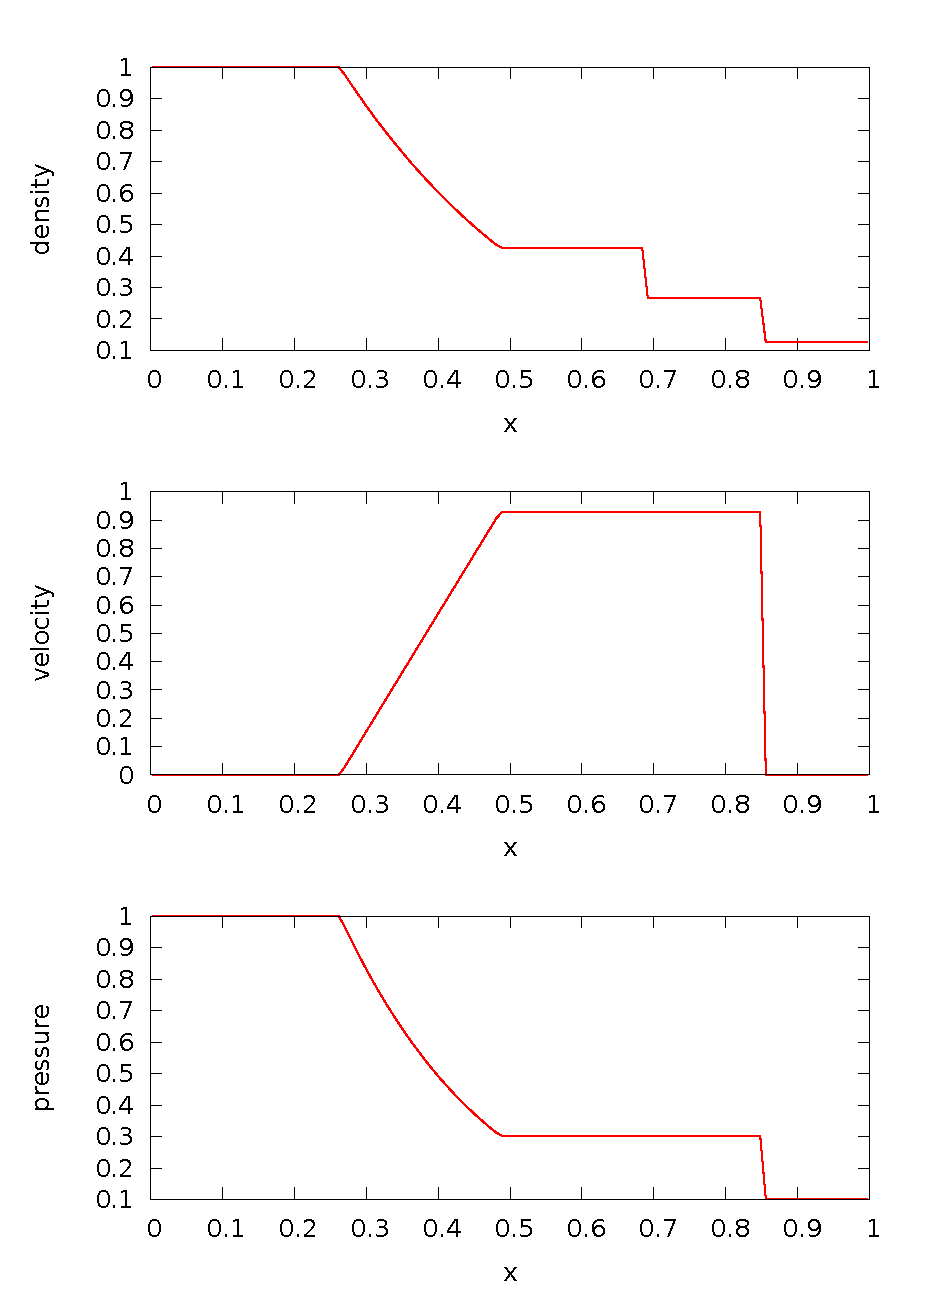
\includegraphics[width=0.8\linewidth]{sod}
\caption[The Sod problem]{\label{fig:sod} Evolution following from an initial
  discontinuity at $x = 0.5$.  These particular conditions are called
  the {\em Sod problem}, and in general, a setup with two states
  separated by a discontinuity is called a shock-tube problem.  We see three
  waves carrying changes in the solution. }
\end{figure}






%-----------------------------------------------------------------------------
\section{The Riemann problem}

Once the interface states are created, the Riemann solver is called.  This
returns the solution at the interface:
\begin{equation}
q_{i+1/2}^{n+1/2} = \mathcal{R}(q_{i+1/2,L}^{n+1/2}, q_{i+1/2,R}^{n+1/2})
\end{equation}

Solving the Riemann problem for the Euler equations can be a complex
operation, but the general ideas are straightforward.  Here we review
the basic outline of operations, and refer to Toro~\cite{toro:1997} for
full details on a variety of methods for solving the Riemann problem.

The Riemann problem consists of a left and right state separated by an
interface.  For the Euler equations, there are three eigenvalues, which
are the speeds at which information propagates.  Each of these
correspond to a wave that will move out from the interface with time,
and each wave will carry with it a jump in the characteristic variables.  The
figure below shows the three waves moving out from the interface,
separating space into 4 regions, marked: $L$, $L^*$, $R^*$, and $R$.
\begin{figure}[h]
\centering
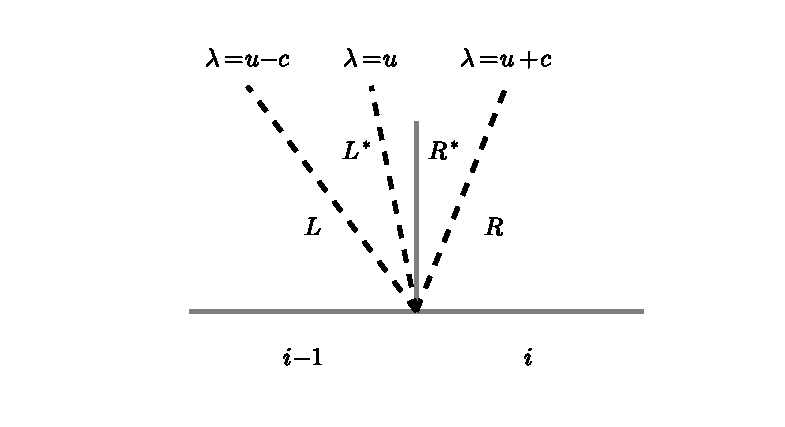
\includegraphics[width=\linewidth]{riemann-waves}
\caption[The Riemann problem wave structure for the Euler
  equations]{The wave structure and 4 distinct regions for the
  Riemann problem.  Time can be thought of as the vertical axis here,
  so we see the waves moving outward from the interface.}
\end{figure}
We typically work in terms of primitive variables.  The states in the
$L$ and $R$ regions are simply the left and right input states---the
waves have not had time to reach here, so they are unmodified.



The middle wave will always be a contact.  We know from the eigenvectors
that the pressure is constant across the contact.

The left and right waves can be either a rarefaction or a shock.  It will
be a shock if the flow is compressive and a rarefaction otherwise.


\subsection{Rarefactions}

The conditions across a rarefaction can be understood by considering
a system where entropy replaces pressure, $q_s = (\rho, u, s)^\intercal$.
The entropy equation is simply $Ds/Dt = 0$.  We need to express the
pressure gradient in the velocity equation in terms of $q_s$.
\begin{equation}
\frac{\partial p(\rho, s)}{\partial x} =
  \left . \frac{\partial p}{\partial s} \right |_\rho \frac{\partial s}{\partial x} +
  \left . \frac{\partial p}{\partial \rho} \right |_s \frac{\partial \rho}{\partial x}
=
  \left . \frac{\partial p}{\partial s} \right |_\rho \frac{\partial s}{\partial x} +
  \frac{p\Gamma_1}{\rho} \frac{\partial \rho}{\partial x}
\end{equation}
giving
\begin{equation}
\frac{\partial u}{\partial t} + u \frac{\partial u}{\partial x} + \frac{1}{\rho} \left [
     \left . \frac{\partial p}{\partial s} \right |_\rho \frac{\partial s}{\partial x} +
          \frac{p\Gamma_1}{\rho} \frac{\partial \rho}{\partial x} \right ] = 0
\end{equation}
This gives a system:
\begin{equation}
{q_s}_t + A_s(q_s) {q_s}_x = 0
\end{equation}
where
\begin{equation}
A_s =
 \left ( \begin{array}{ccc} u & \rho & 0 \\
        c^2/\rho & u & \frac{1}{\rho} \left . \frac{\partial p}{\partial s}\right |_\rho \\
        0 & 0 & u \end{array} \right )
\end{equation}
The eigenvalues of $A_s$ are again $u$, $u-c$, and $u+c$.  The right eigenvectors
are\footnote{Again, see the {\sf SymPy} {\sf IPython} notebook:
\hydroexdoit{\href{https://github.com/zingale/hydro_examples/blob/master/compressible/euler.ipynb}{euler.ipynb}}}
\begin{align}
r_s^\evm = \left ( \begin{array}{c} 1 \\ -c/\rho \\ 0 \end{array} \right )
%
\qquad
r_s^\evz = \left ( \begin{array}{c} 1 \\ 0 \\ -c^2/p_s  \end{array} \right )
%
\qquad
r_s^\evp = \left ( \begin{array}{c} 1 \\ c/\rho \\ 0 \end{array} \right )
\end{align}
Since the jump in $q_s$ is proportional to these eigenvectors, we see that
entropy does not change across the left, $(-)$, and right, $(+)$, waves.


\subsection{Shocks}

Entropy is not constant across a shock---there is dissipation, so we
need a different way to connect the states across the shock.  As with
Burgers' equation, we can understand the shock by looking at the
Rankine-Hugoniot jump conditions.  There will be one condition for
each of our conservation laws, and together they tell us the speed of
the shock and how density and pressure jump across
it.  \MarginPar{derive jump conditions}

The left and right states are connected to the state in the star
region by a Hugoniot curve---this is a curve in the $u$-$p$ plane that
shows all of the possible states one can reach from the current state
through either a shock or rarefaction.  There are two such curves, one
corresponding to the left and one to the right state, and the solution
to the Riemann problem is the point in the $u$-$p$ plane where these
two curves intersect.  Figure~\ref{fig:euler:riemann-curve} shows the
Hugoniot curves for the Sod problem.

\begin{figure}[t]
\centering
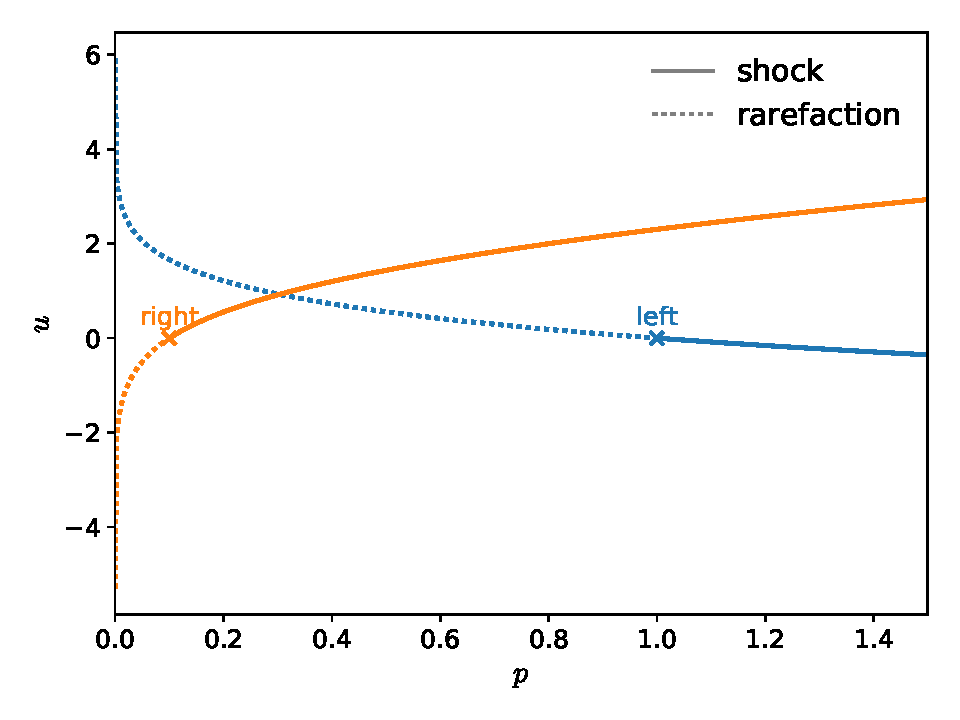
\includegraphics[width=0.9\linewidth]{riemann-phase}
\caption[The Hugoniot curves corresponding
to the Sod problem]{\label{fig:euler:riemann-curve} The Hugoniot
curves corresponding to the Sod problem.  The shock and rarefaction
curves are shown.  The solution to the Riemann problem is the point
where the curves intersect.\\
\hydroexdoit{\href{https://github.com/zingale/hydro_examples/blob/master/compressible/riemann-phase.py}{riemann-phase.py}}}
\end{figure}


\subsection{Interface solution}

We are interested in the state at the interface.  To
determine this, we need to determine which region we are in.  That
requires an estimation of the wave speeds.  Since these are nonlinear
waves, we cannot in general just use the eigenvalues (although some
approximate solvers do).  Different Riemann solvers will have
different approximations for finding the speeds of the left, center,
and right wave.  Note the figure shows only one possible configuration
for the waves---they can all be on one side of the interface (for
all supersonic waves), or the contact (the middle wave) can be on either
side.

Once the wave speeds are known, we look at the sign of the speeds to
determine which of the 4 regions is on the interface.  In the `star'
region, only $\rho$ jumps across the middle (contact) wave, the
pressure and velocity are constant across that wave (see $r^\evz$).
We determine the state in the star region ($\rho_l^*, \rho_r^*, u^*,
p^*$) by using the jump conditions for the Euler equations.  In
general, these differ depending on whether the waves are shocks or
rarefactions.  In practice, approximate Riemann solvers often assume
one or the other (for example, the two-shock Riemann solver used
in~\cite{colellaglaz:1985}).  With the wave speeds and the states
known in each region, we can evaluate the state on the interface,
$q_{i+1/2}^{n+1/2}$.

Recall that a rarefaction involves diverging flow---it spreads out
with time.  Special consideration needs to be taken if the rarefaction
wave spans the interface (a {\em transonic rarefaction}).  In this
case, most Riemann solvers interpolate between the left or right state
and the appropriate star state.

Then the fluxes are computed from this state as:
\begin{equation}
\renewcommand{\arraystretch}{1.5}
F_{i+1/2}^{n+1/2} = \left ( \begin{array}{c}
                             \rho_{i+1/2}^{n+1/2} u_{i+1/2}^{n+1/2} \\
                             \rho_{i+1/2}^{n+1/2} (u_{i+1/2}^{n+1/2})^2 + p_{i+1/2}^{n+1/2} \\
                             u_{i+1/2}^{n+1/2} p_{i+1/2}^{n+1/2} / (\gamma - 1)  +
                             \frac{1}{2} \rho_{i+1/2}^{n+1/2} (u_{i+1/2}^{n+1/2})^3 +
                             u_{i+1/2}^{n+1/2} p_{i+1/2}^{n+1/2}
                            \end{array} \right )
\renewcommand{\arraystretch}{1.0}
\end{equation}

Note that instead of returning an approximate state at the interface,
some Riemann solvers (e.g.\ the HLL(C) solvers) instead approximate the
fluxes directly.  These use estimates of the wave speeds together with
the Rankine-Hugoniot jump conditions to give the fluxes.



%-----------------------------------------------------------------------------
\section{Other Thermodynamic Equations}

At times we will want to use alternate forms of the energy equation.  The
internal energy is governed by the first law of thermodynamics.  In the
absence of any heat sources, we have:
\begin{equation}
dq = 0 = de + pd(1/\rho)
\end{equation}
where $e$ is the specific internal energy.
Applying this to a Lagrangian fluid element, we have:
\begin{align}
\frac{De}{Dt} + p \frac{D(1/\rho)}{Dt} &= 0 \\
\frac{De}{Dt} - \frac{p}{\rho^2} \frac{D\rho}{Dt} &= 0 \\
\rho \frac{De}{Dt} + p \nabla \cdot U &= 0
\end{align}
where we used the continuity equation in the last step to eliminate
$D\rho/Dt$.  This can be rewritten by adding $e \times$ the continuity
equation to give:
\begin{equation}
\frac{\partial (\rho e)}{\partial t} + \nabla \cdot (\rho U e) + p \nabla \cdot U = 0 \label{eq:euler:econs}
\end{equation}


\subsection{Eigensystem with Temperature}

Here we illustrate how the eigensystem changes when we replace pressure with
temperature in our primitive variable system.

We write this set of variables as $\hat{q} = (\tau, u,
T)^\intercal$---note that we keep $\tau$ instead of $\rho$ here.  The
motivation for this comes from the fact that with temperature in the
mix, the temperature will jump across the contact wave.  Since
pressure should be constant across the contact, and, even with the
general EOS, a temperature jump needs a density drop for pressure to
remain constant, $\tau$ should counteract the behavior of $T$ across
the contact.

The temperature evolution equation appears as:
\begin{equation}
\frac{\partial T}{\partial t} = -u\ddx{T} +
  \frac{1}{\rho c_p} \left [ (1 - \rho h_p) \frac{Dp}{Dt} \right ]
\end{equation}
(see, e.g.\ \cite{ABRZ:I}) where $c_p$ is the specific heat at
constant pressure, $c_p = \partial h/\partial T|_p$ and $h_p \equiv
\partial h / \partial p |_T$, with $h = e + p/\rho$ the specific
enthalpy.  We can use the standard pressure evolution equation
(Eq.~\ref{eq:euler:pgeneral}) to eliminate the Lagrangian pressure term,
resulting in:
\begin{equation}
\frac{\partial T}{\partial t} = -u\ddx{T} - \eta \ddx{u}
\end{equation}
where we defined
\begin{equation}
\eta \equiv \frac{1 - \rho h_p}{c_p} c^2
\end{equation}

The density equation remains unchanged from the traditional primitive
variable formulation, but for the velocity, we need to write the
$\partial p/\partial x$ term in terms of $\hat{q}$.  We do this via
the chain rule.  We define $p_\rho \equiv {\partial p}/{\partial \rho}
|_T$ and $p_T \equiv {\partial p}/{\partial T} |_\rho$, then our
velocity equation is:
\begin{equation}
\frac{\partial u}{\partial t} + u \frac{\partial u}{\partial x} - \frac{p_\rho}{\tau} \frac{\partial \tau}{\partial x} + {\tau p_T} \frac{\partial T}{\partial x} = 0
\end{equation}
Note that here we neglected any composition dependence in the EOS.

Our primitive variable system in matrix form is then:
\begin{equation}
\hat{q}_t + \hat{A} \hat{q}_x = 0
\end{equation}
with
\begin{equation}
\renewcommand{\arraystretch}{1.5}
\hat{A}(\hat{q}) =
\left (
\begin{array}{ccc}
u                   & -\tau & 0 \\
-\dfrac{p_\rho}{\tau} & u    & \tau p_T \\
0                   & \eta & u
\end{array}
\right )
\end{equation}
The eigenvalues can be found through the characteristic polynomial,
$|\hat{A} - \lambda I| = 0$:
\begin{equation}
(u - \lambda)^3 - (u -\lambda) \left ( {p_T \eta\tau} + p_\rho \right ) = 0
\end{equation}
We can simplify the last term in parenthesis:
\begin{equation}
{p_T \eta\tau} + p_\rho = \frac{p_T (1 - \rho h_p) c^2}{\rho c_p} + p_\rho
                               = \frac{c^2}{c_p}\left ( \frac{p p_T}{\rho^2 p_\rho} - \frac{p_T e_\rho}{p_\rho} \right ) + p_\rho \label{eq:step1}
\end{equation}
where we substituted in
\begin{equation}
h_p = \frac{1}{\rho} \left ( 1 - \frac{p}{\rho p_\rho} \right ) + \frac{e_\rho}{p_\rho}
\end{equation}
(see \cite{ABRZ:I}, appendix A) where $e_\rho = \partial e/\partial
\rho |_T$.  The term in parenthesis in Eq.~\ref{eq:step1} is simply
$c_p - c_v$ (\cite{cg}, Eq.~9.81) where $c_v$ is the specific heat
at constant volume, and Eq.~\ref{eq:step1} further reduces to:
\begin{equation}
{p_T \eta\tau} + p_\rho = \frac{c^2}{c_p} (c_p - c_v) + p_\rho
                               = c^2 - c^2 \frac{\chi_p}{\Gamma_1} + p_\rho = c^2
\end{equation}
where we used $c_v/c_p = \chi_p/\Gamma_1$ and $\chi_p = \rho p_\rho /
p$ (\cite{cg}, Eqs.~9.87, 9.82).  Putting this into our
characteristic polynomial, we see that the eigenvalues are, as expected,
$\lambda = u, u \pm c$.  It is also useful to note that
\begin{equation}
\eta = \frac{c^2 - p_\rho}{\tau p_T}
\end{equation}


We construct the left and right eigenvectors such that they are orthonormal,
and find:
\begin{equation}
\renewcommand{\arraystretch}{1.3}
\hat{R} = \left ( \begin{array}{ccc}
     1                       & 1                 & 1 \\
   c/\tau                    & 0                 & -c/\tau \\
  -(c^2 - p_\rho)/\tau^2 p_T & p_\rho/\tau^2 p_T & -(c^2 - p_\rho)/\tau^2 p_T
  \end{array} \right )
\end{equation}
and
\begin{equation}
\hat{L} = \left ( \begin{array}{ccc}
      {p_\rho}/{2 c^2}   & {\tau}/{2c}  & -{\tau^2 p_T}/{2 c^2} \\
      1 - {p_\rho}/{c^2} &0             & {\tau^2 p_T}/{c^2} \\
      {p_\rho}/{2 c^2}   & -{\tau}/{2c} & -{\tau^2 p_T}/{2 c^2} \end{array} \right )
\end{equation}
We note that all
thermodynamic derivatives are expressed in terms of $\rho$ or $T$ with
the other quantity held constant.  This is in the form we expect a
$(T, \rho)$-based EOS to return derivatives.  Notice also that the
temperature jumps across the $\evz$ wave (the contact discontinuity;
this is seen from the non-zero value in $\hat{r}^\evz$ for the
temperature).

We write:
\begin{eqnarray}
\hat{\beta}^\evm_s &\equiv& (\hat{l}^\evm \cdot \Delta \hat{q}^\evm ) =
   \frac{1}{2C} \left (\frac{\rho^2 p_\rho}{C} \Delta \tau^\evm
                        + \Delta u^\evm - \frac{p_T}{C}\Delta T^\evm \right ) \\
%
\hat{\beta}^\evz_s &\equiv& (\hat{l}^\evz \cdot \Delta \hat{q}^\evz ) =
    \Delta \tau^\evz +
        \frac{1}{C^2} \left (-\rho^2 p_\rho \Delta \tau^\evz
                        + {p_T}\Delta T^\evz \right ) \\
%
\hat{\beta}^\evp_s &\equiv& (\hat{l}^\evp \cdot \Delta \hat{q}^\evp ) =
   \frac{1}{2C} \left (\frac{\rho^2 p_\rho}{C} \Delta \tau^\evp
                        - \Delta u^\evp - \frac{p_T}{C}\Delta T^\evp \right )
\end{eqnarray}
Note that since $p_\tau = -\rho^2 p_\rho$, we can form a $\Delta p^\enu$ as
\begin{equation}
\Delta p^\enu = p_\tau \Delta \tau^\enu + p_T \Delta T^\enu
\end{equation}
and then we see that the $\hat{\beta}^\enu$'s above have the same
functional form as the $\mathring{\beta}^\enu$ from the $\mathring{q}
= (\tau, u, p, e)^\intercal$ eigensystem.  This is no surprise, since
the $l\cdot \Delta q$ are the characteristic variables of the Euler
equations.  The numerical values will differ though, because the
$\hat{\beta}^\enu$ and $\mathring{\beta}^\enu$ use different reference
states and reconstructed variables.

Finally, we can write out the interface states:
\begin{eqnarray}
\tau_s &=& \tilde{\tau} - (\hat{\beta}^\evm + \hat{\beta}^\evz + \hat{\beta}^\evp) \\
%
u_s &=& \tilde{u} - (C \hat{\beta}^\evm - C \hat{\beta}^\evp) \\
%
T_s &=& \tilde{T} - \frac{1}{p_T} \left \{
   \left [ -C^2 \hat{\beta}^\evm - C^2 \hat{\beta}^\evp \right ] +
   \rho^2 p_\rho \left [ \hat{\beta}^\evm + \hat{\beta}^\evz + \hat{\beta}^\evp \right ] \right \}
\end{eqnarray}
For $T_s$, we recognize the first quantity in the square brackets as
being the same as $-(p_s - \tilde{p})$ in the $\mathring{q}$ system, and the
second term in the square brackets being the same as $-(\tau_s - \tilde{\tau})$
in the $\mathring{q}$ system, then we see
\begin{equation}
p_T (T_s - \tilde{T} ) \approx (p_s - \tilde{p} ) - p_\tau (\tau_s - \tilde{\tau})
\end{equation}
which is what we would expect for jumps in $p$ when applying the chain
rule.  Note that this is not a strict equality, since the reference
states and interpolation between the two eigensystems are different.
Nevertheless, this demonstrates the connection between the two
methods.

The above did not consider variations in the composition of the fluid.
Multiple species complicate things---now the replacement of the
pressure gradient picks up a composition gradient term.
The eigensystem will change with this addition.  We don't explore this here at this
time.

